\chapter{Supervised learning}
\minitoc
\begin{kwd}
Bayes classifier, empirical risk, oracle inequality, linear discriminant analysis, logistic regression.
\end{kwd}


In a supervised learning framework, a set $\{(X_i,Y_i)\}_{1\leqslant i \leqslant n}$  of input data (also referred to as {\em features}) $X_i\in\xset$ and output data $Y_i\in\yset$ (also referred to as {\em observations}), for $1\leqslant i \leqslant n$, is available, where $\xset$ is a general feture space and $\yset$ is a general observation space. In a supervised classification setting, the problem is to learn wether an individual from a given state space $\xset$ belongs to some class, so that $\yset = \{1,\ldots,M\}$ for some $M\geqslant 1$. In a regression framework, the observation set $\yset$ is usually a subset of $\rset^m$. The state space $\xset$ is usually a subset of $\rset^d$ and an element of $\xset$ contains all the features the observation prediction is  based on.

One of the main goals of supervised learning is to design an automatic procedure, based on  the {\em training dataset} $\{(X_i,Y_i)\}_{1\leqslant i \leqslant n}$,  to predict the observation $y\in\yset$ associated with an input $x\in\xset$ which is not in the training dataset.

\medskip

The simulations presented in these notes can be found at \url{https://sylvainlc.github.io/}. Most elementary numerical solutions are based on scikit-learn, the website \url{https://scikit-learn.org/stable/supervised\_learning.html} provides many helpful comments and advices.


\section{Losses and risks}
In these notes, we consider that $\{(X_i,Y_i)\}_{1\leqslant i \leqslant n}$ are independent and identically distributed (i.i.d.) with the same distribution as a couple of random variables $(X,Y)$ defined on  a measured space $(\Omega,\calF,\bP)$ and taking values in $\xset\times\yset$. The joint distribution of $(X,Y)$ is unknown. A loss function is used to evaluate the prediction of the observations: $\ell: \yset\times \yset \to \rset$.
\begin{itemize}
\item In a classification setting where $\yset = \{1,\ldots,M\}$ for some $M\geqslant 1$, a common loss function is $\ell : (y,y')\mapsto \1_{y\neq y'}$. This 0-1 loss outputs 1 if the prediction $y'\in\yset$ is different from the true class $y\in\yset$.
\item In a regression setting,  common loss functions are $\ell : (y,y')\mapsto \|y-y'\|_2^2$ and $\ell : (y,y')\mapsto \|y-y'\|_1$.
\end{itemize}
Once the loss function is chosen, the expected risk allows to evaluate all predictors $f: \xset\to \yset$. It is defined  as the expected loss between the observation $Y$ and the prediction $f(X)$:
$$
\mathsf{R}(f) = \bE\left[\ell(Y,f(X))\right]\eqsp.
$$
\begin{itemize}
\item In a classification setting using the 0-1 loss, the risk function is $\mathsf{R}_{}(f) = \bE\left[\1_{Y\neq h(X)}\right]= \bP(Y\neq f(X))$. It is also known as the {\em misclassification loss}.
\item In a regression setting using the square loss,   the risk function is $\mathsf{R}(f) = \bE[\|Y-f(X)\|^2_2]$.
\end{itemize}
This risk is typically unknown as the joint distribution of $(X,Y)$ is unknown, i.e. the expectation cannot be computed explicitly. Therefore, a classical surrogate is given by the empirical risk:
$$
\mathsf{R}_n(f) = \frac{1}{n}\sum_{i=1}^n\ell(Y_i,f(X_i))\eqsp.
$$
In empirical risk minimization, we often define a parameterized family of predictors $\{f_\param\}_{\param\in \paramset}$ where $\paramset\in \rset^q$ and for all $\param\in\paramset$, $f_\param: \xset\to \yset$ and seek to minimize the empirical risk over this parameterized family:
$$
\widehat\param_n \in\argmin_{\param\in\paramset} \left\{\mathsf{R}_n(f_\param) = \frac{1}{n}\sum_{i=1}^n\ell(Y_i,f_\param(X_i)) \right\}\eqsp.
$$

\subsection*{Cross-validation (see also Section~\ref{sec:ridge:choicepen})} 
In practice, several parameterized families of predictors can be considered to minimize the empirical risk. Each parameterized family provides an empirical best predictor. Cross-validation (CV) provides appealing strategies for algorithm selection. Cross-validation proposes to split the data to estimate the risk of each algorithm: part of data  is used  to train each
algorithm (or minimize the empirical risk over each parameterized family), and the remaining part is used to estimate
the risk of the estimated predictor.  In \cite{arlot2010survey}, the authors provide a survey of the most common cross-validation techniques and a few  guidelines to choose the best technique depending on the statistical learning setting. 

The most widespread technique is probably the $k$-fold cross-validation approach, see \cite{geisser1975predictive}. In this case, the training dataset is first randomly  partitioned into $k$ subset $\mathcal{D}_i$, $1\leqslant i \leqslant k$. Each subset $\mathcal{D}_i$, $1\leqslant i \leqslant k$,  is iteratively removed from the dataset before training the algorithm. Then, the empirical risk of the trained algorithm is computed over $\mathcal{D}_i$. The estimated risk of the algorithm is given by the empirical mean of the risks obtained  when each $\mathcal{D}_i$, $1\leqslant i \leqslant k$, is removed from the training dataset and used to evaluate the risk. Additional details and illustrations can be found for instance here: \url{https://scikit-learn.org/stable/modules/cross\_validation.html}.


\section{Bayes classifier}
\index{Bayes!classifier}
Let $(\Omega,\calF,\bP)$ be a probability space. Assume that $(X,Y)$ is a couple of random variables defined on  $(\Omega,\calF,\bP)$ and taking values in $\xset\times\{-1,1\}$ where $\xset$ is a given state space, which means that the focus is set on a two-class classification problem. One aim of supervised classification is to define a function $h: \xset \to \{-1,1\}$, called {\em classifier}, such that $h(X)$ is the best prediction of $Y$ in a given context. For instance, the risk of misclassification of $h$ is \index{classification risk}
\[
\mathsf{R}_{\mathrm{miss}}(h) = \bE\left[\1_{Y\neq h(X)}\right] =  \bP\left(Y\neq h(X)\right)\eqsp.
\]
Note that $\bE[Y|X]$ is a random variable measurable with respect to the $\sigma$-algebra $\sigma(X)$. Therefore, there exists a function $\eta:\xset \to [-1,1]$ so that $\bE[Y|X] = \eta(X)$ almost surely.
\begin{shaded}
\begin{lemma} \label{lem:bayesclassif}
The classifier $h_{\star}$, defined for all $x\in\xset$, by
\[
h_{\star}(x) = \left\{
    \begin{array}{ll}
       1 & \mbox{if }\; \eta(x)>0\eqsp, \\
        -1 & \mbox{otherwise}\eqsp,
    \end{array}
\right.
\]
is such that
\[
h_{\star} = \underset{h:\xset\to\{-1,1\}}{\argmin}\mathsf{R}_{\mathrm{miss}}(h)\eqsp.
\]
\end{lemma}
\end{shaded}
\begin{proof}
For all $u,v \in \{-1,1\}$, $\indin{u \neq v}=\indin{u v=-1}=(1-uv)/2$. Since $Y$ and $h(X)$ take values in $\{-1,1\}$, this implies
\begin{equation} \label{eq:miss}
\Lmiss(h)=\PP(Y\neq h(X)) = \left(1-\PE[Y h(X)]\right)/2\eqsp.
\end{equation}
Using sucessively the tower property, the equality $|u|= u\times \sgn(u)$, and the tower property again yields
$$
\PE[Y h(X)] =\PE[\CPE{Y}{X} h(X)] \leq \PEs{|\CPE{Y}{X}| \underbrace{|h(X)|}_{=1}}=  \PEs{\CPE{Y}{X} \underbrace{\sgn(\CPE{Y}{X})}_{h_\star(X)}}=\PE[Y h_\star(X)]\eqsp.
$$
Plugging this into \eqref{eq:miss} yields $\Lmiss(h) \geq \Lmiss(h_\star)$, which concludes the proof.
\end{proof}
%\begin{proof}
%Let $h:\xset\to\{-1,1\}$. First note that, as $Y$ and $h(X)$ take values in $\{-1,1\}$,
%\[
%\bE\left[(Y-h(X))^2\right] = \bE\left[(Y-h(X))^2\1_{Y\neq h(X)}\right] = 4  L_{\mathrm{miss}}(h)\eqsp.
%\]
%Therefore,
%\[
%\underset{h:\xset\to\{-1,1\}}{\argmin} L_{\mathrm{miss}}(h)= \underset{h:\xset\to\{-1,1\}}{\argmin}\bE\left[(Y-h(X))^2\right] \eqsp.
%\]
%Then, write
%\[
%\bE\left[(Y-h(X))^2\right] = \bE\left[(Y-\bE[Y|X])^2\right] + \bE\left[(\bE[Y|X] - h(X))^2\right] + 2\bE\left[(Y-\bE[Y|X])(\bE[Y|X] - h(X))\right]\eqsp.
%\]
%To deal with the last term, since $\bE[Y|X] - h(X)$ is measurable with respect to $\sigma(X)$,
%\begin{align*}
%\bE\left[(Y-\bE[Y|X])(\bE[Y|X] - h(X))\right] &= \bE\left[\bE\left[(Y-\bE[Y|X])(\bE[Y|X] - h(X))\middle | X\right]\right]\eqsp,\\
% &= \bE\left[(\bE[Y|X] - h(X))\bE\left[(Y-\bE[Y|X])\middle | X\right]\right]\eqsp,\\
% &= \bE\left[(\bE[Y|X] - h(X))(\bE\left[Y\middle |X\right]-\bE[Y|X])\right]\eqsp,\\
%&=0\eqsp.
%\end{align*}
%This yields
%\[
%\underset{h:\xset\to\{-1,1\}}{\argmin} L_{\mathrm{miss}}(h)= \underset{h:\xset\to\{-1,1\}}{\argmin} \bE\left[(\bE[Y|X] - h(X))^2\right]\eqsp.
%\]
%Since $h(X)\in\{-1,1\}$, expanding the square inside the expectation, we get
%$$
%\bE\left[(\bE[Y|X] - h(X))^2\right]=\bE\left[\bE[Y|X]^2\right]+1 -2 \bE\left[\bE[Y|X]h(X)\right]
%$$
%The minimum is thus obtained by setting $\bE[Y|X]h(X)=|\bE[Y|X]|$, that is by taking $h(X)$ as the sign of $\bE[Y|X]$.
%\end{proof}
Note that
\[
\bE\left[Y\middle |X\right] = \bP\left(Y=1\middle|X\right) - \bP\left(Y=-1\middle|X\right) = 2\bP\left(Y=1\middle|X\right) -1\eqsp,
\]
which motivates this alternative definition of $h_{\star}$.
\begin{shaded}
\begin{definition} \label{def:bayesclassif}
The classifier $h_{\star}$ is called the Bayes classifier. It may also be written as follows:
\[
h_{\star}(X) = \left\{
    \begin{array}{ll}
       1 & \mbox{if }\; \bP\left(Y=1\middle|X\right)>1/2 \mbox{ i.e. if } \CPP{Y=1}{X}>\CPP{Y=-1}{X}\eqsp, \\
        -1 & \mbox{otherwise}\eqsp.
    \end{array}
\right.
%=\begin{cases}
%1 & \mbox{if $\CPP{Y=1}{X}>\CPP{Y=-1}{X}$}\eqsp,\\
%-1 & \mbox{otherwise}\eqsp,
%\end{cases}
\]
\end{definition}
\end{shaded}
%Definition~\ref{def:bayesclassif} is a direct consequence of
%\[
%\bE\left[Y\middle|X\right] = \bP\left(Y=1\middle|X\right) - \bP\left(Y=-1\middle|X\right) = 2 \bP\left(Y=1\middle|X\right) - 1 \eqsp.
%\]
The Bayes classifier is the optimal choice to minimize the probability of misclassification $\Lmiss$. However, as the conditional distribution of $Y$ given $X$ is usually unknown, it cannot be computed explicitly. Supervised classification aims at designing an approximate classifier $\widehat h_n$ using independent observations $(X_i,Y_i)_{1\leqslant i\leqslant n}$ with the same distribution as $(X,Y)$ so that the error $\Lmiss(\widehat h_n)-\Lmiss(h_{\star})$ may be controlled.

\section{Parametric and semiparametric classifiers}
\subsection{Mixture of Gaussian distributions}
\index{models!parametric}
In this first example, we consider a {\em parametric model}, that is, we assume that the joint distribution of $(X,Y)$ belongs to a family of distributions parametrized by a vector $\theta$ with real components. For $k\in\{-1,1\}$, write $\pi_k = \bP(Y = k)$. Assume that $\xset = \rset^d$ and that, conditionally on the event $\{Y = k\}$, $X$ has a Gaussian distribution with mean $\mu_k \in\rset^d$ and covariance matrix $\Sigma\in \rset^{d\times d}$, whose density is denoted $g_k$. In this case, the parameter $\theta=(\pi_1, \mu_1,\mu_{-1}, \Sigma)$ belongs to the set $\Theta= [0,1] \times \rset^d \times \rset^d \times \rset^{d \times d}$. The parameter $\pi_{-1}$ is not part of the components of $\theta$ since $\pi_{-1}=1-\pi_{1}$. In this case, the parameter $\theta=(\pi_1, \mu_1,\mu_{-1}, \Sigma)$ belongs to the set $\Theta= [0,1] \times \mathbb{R}^d \times \mathbb{R}^d \times \mathbb{R}^{d \times d}$. The parameter $\pi_{-1}$ is not part of the components of $\theta$ since $\pi_{-1}=1-\pi_{1}$. The explicit computation of $\mathbb{P}(Y=1 | X)$ writes
$$
\mathbb{P}\left(Y=1\middle | X\right) = \frac{\pi_1g_1(X)}{\pi_1g_1(X) + \pi_{-1}g_{-1}(X)} = \frac{1}{1 + \frac{\pi_{-1}g_{-1}(X)}{\pi_1g_1(X)}} = \sigma\left(\log(\pi_1/\pi_{-1}) + \log(g_1(X)/g_{-1}(X)\right)\,,
$$
where $\sigma: x\mapsto (1 + \mathrm{e}^{-x})^{-1}$ is the sigmoid function. Then,
\begin{equation}
\label{eq:prob:lda}
\mathbb{P}\left(Y=1\middle | X\right) = \sigma\left( X^\top\omega+ b\right)\eqsp,
\end{equation}
where
$$
\omega =  \Sigma^{-1}\left(\mu_{1} - \mu_{-1}\right)\,,
b = \log(\pi_1/\pi_{-1}) +  \frac{1}{2}\left(\mu_{1}+\mu_{-1}\right)^\top\Sigma^{-1}\left(\mu_{-1}-\mu_{1}\right)\eqsp.
$$
Since
\[
\bE\left[Y\middle| X\right]  = \bP\left(Y=1\middle | X\right) - \bP\left(Y=-1\middle | X\right)\eqsp,
\]
the Bayes classifier is such that for all $x\in \xset$,
\begin{align*}
h_{\star}(x) = 1%& \Leftrightarrow \left. \bP\left(Y=1\middle | X\right)\right|_{X=x} > \left. \bP\left(Y=-1\middle | X\right) \right|_{X=x}\eqsp,\\
& \Leftrightarrow \pi_1 \exp\left\{-\frac{1}{2}\left(x-\mu_1\right)^\top\Sigma^{-1}\left(x-\mu_1\right)\right\} > \pi_{-1} \exp\left\{-\frac{1}{2}\left(x-\mu_{-1}\right)^\top\Sigma^{-1}\left(x-\mu_{-1}\right)\right\}\eqsp,\\
& \Leftrightarrow \log\left(\frac{\pi_{1}}{\pi_{-1}}\right) > -\frac{1}{2}\left(x-\mu_{-1}\right)^\top\Sigma^{-1}\left(x-\mu_{-1}\right) + \frac{1}{2}\left(x-\mu_1\right)^\top\Sigma^{-1}\left(x-\mu_1\right)\eqsp,\\
& \Leftrightarrow \log\left(\frac{\pi_{1}}{\pi_{-1}}\right) > x^\top \Sigma^{-1}\left(\mu_{-1} - \mu_{1}\right) + \frac{1}{2}\left(\mu_{1}+\mu_{-1}\right)^\top\Sigma^{-1}\left(\mu_{1}-\mu_{-1}\right)\eqsp.
\end{align*}
In this case, the Bayes classifier is given by
\[
h_{\star}: x\mapsto  \left\{
    \begin{array}{ll}
       1 & \mbox{if }\; \left\langle \Sigma^{-1}\left(\mu_1-\mu_{-1}\right);x - \frac{\mu_1  +\mu_{-1}}{2}\right\rangle + \log\left(\frac{\pi_{1}}{\pi_{-1}}\right)>0\eqsp, \\
        -1 & \mbox{otherwise}\eqsp,
    \end{array}
\right.
\]
\begin{figure}
\begin{center}
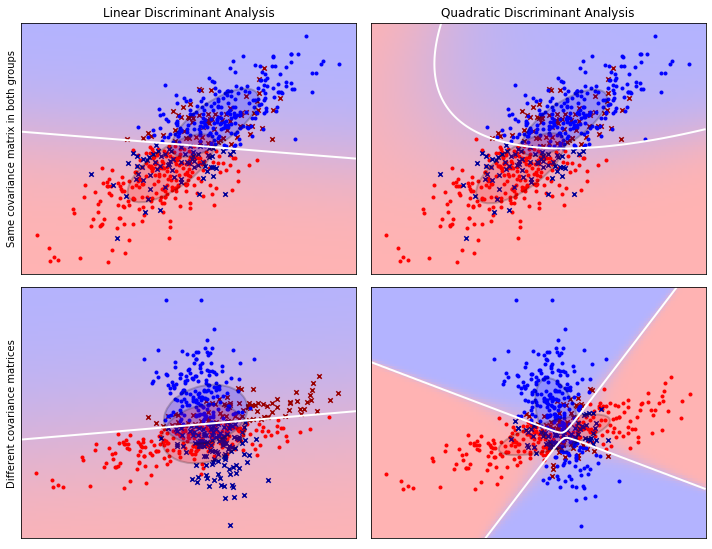
\includegraphics[width = .8\linewidth]{./Illustrations/lda_plot.png}
\end{center}
\caption{(Top) Data are generated with the same covrariance matrix in each group. (Bottom) Data are generated with different covrariance matrices in the two groups.  (Left) Classification boundary obtained with LDA, assuming the covariance matrix is the same in each group. (Right)  Classification boundary obtained with QDA, assuming the covariance matrices are different in each group. Crosses are all false positives i.e. all data wrongly classified by the discriminant analysis. Simulations are inspired by \url{https://scikit-learn.org/stable/modules/lda_qda.html\#mathematical-formulation-of-the-lda-and-qda-classifiers} and can be found here \url{https://sylvainlc.github.io/}.}
\end{figure}
Additional numerical considerations can be found for instance here \url{https://scikit-learn.org/stable/modules/lda_qda.html#mathematical-formulation-of-the-lda-and-qda-classifiers}.


When $\Sigma$ and $\mu_1$ and $\mu_{-1}$ are unknown, this classifier cannot be computed explicitely. We will approximate it using the observations. Assume that  $(X_i,Y_i)_{1\leqslant i\leqslant n}$ are independent observations with the same distribution as $(X,Y)$. The loglikelihood of these observations is given by
\begin{align*}
\log \bP_{\theta}\left(X_{1:n},Y_{1:n}\right) &=\sum_{i=1}^n \log \bP_{\theta} \left(X_{i},Y_{i}\right)\eqsp,\\
&= - \frac{nd}{2} \log(2\pi)+\sum_{i=1}^n\sum_{k\in\{-1,1\}}\1_{Y_i=k}\left(\log \pi_{k} -\frac{\log \det \Sigma}{2} - \frac{1}{2}\left(X_i - \mu_{k}\right)^\top\Sigma^{-1}\left(X_i - \mu_{k}\right)\right) \eqsp,\\
&= - \frac{nd}{2} \log(2\pi)-\frac{n}2 \log\det\Sigma + \left(\sum_{i=1}^n\1_{Y_i=1}\right)\log \pi_1 + \left(\sum_{i=1}^n\1_{Y_i=-1}\right)\log (1-\pi_{1})\\
& \hspace{1cm}-  \frac{1}{2}\sum_{i=1}^n\1_{Y_i=1}\left(X_i - \mu_{1}\right)^\top\Sigma^{-1}\left(X_i - \mu_{1}\right) -  \frac{1}{2}\sum_{i=1}^n\1_{Y_i=-1}\left(X_i - \mu_{-1}\right)^\top\Sigma^{-1}\left(X_i - \mu_{-1}\right)\eqsp.
\end{align*}
By Lemma~\ref{lem:matrix:calculus}, the gradient of $\log \bP_{\theta}\left(X_{1:n},Y_{1:n}\right)$ with respect to $\theta$ is therefore given by
\begin{align*}
\frac{\partial \log \bP_{\theta}\left(X_{1:n},Y_{1:n}\right)}{\partial \pi_1} &= \left(\sum_{i=1}^n\1_{Y_i=1}\right)\frac{1}{\pi_1} - \left(\sum_{i=1}^n\1_{Y_i=-1}\right)\frac{1}{1-\pi_{1}}\eqsp,\\
\frac{\partial \log \bP_{\theta}\left(X_{1:n},Y_{1:n}\right)}{\partial \mu_1} &= \sum_{i=1}^n\1_{Y_i=1}\left(2\Sigma^{-1}X_i - 2\Sigma^{-1}\mu_{1}\right)\eqsp,\\
\frac{\partial \log \bP_{\theta}\left(X_{1:n},Y_{1:n}\right)}{\partial \mu_{-1}} &= \sum_{i=1}^n\1_{Y_i=-1}\left(2\Sigma^{-1}X_i - 2\Sigma^{-1}\mu_{-1}\right)\eqsp,\\
\frac{\partial \log \bP_{\theta}\left(X_{1:n},Y_{1:n}\right)}{\partial \Sigma^{-1}} &= \frac{n}{2}\Sigma -  \frac{1}{2}\sum_{i=1}^n\1_{Y_i=1}\left(X_i - \mu_{1}\right)\left(X_i - \mu_{1}\right)^\top -  \frac{1}{2}\sum_{i=1}^n\1_{Y_i=-1}\left(X_i - \mu_{-1}\right)\left(X_i - \mu_{-1}\right)^\top\eqsp.
\end{align*}
The maximum likelihood estimator is defined as the only parameter $\widehat \theta^n$ such that all these equations are set to 0. For $k\in\{-1,1\}$,  it is given by
\begin{align*}
\widehat \pi_k^n &= \frac{1}{n}\sum_{i=1}^n\1_{Y_i=k}\eqsp,\\
\widehat \mu_k^n &= \frac{1}{\sum_{i=1}^n\1_{Y_i=k}}\sum_{i=1}^n\1_{Y_i=k}\,X_i\eqsp,\\
\widehat\Sigma^n &= \frac{1}{n}\sum_{i=1}^n \left(X_i - \widehat \mu_{Y_i}^n\right)\left(X_i - \widehat \mu_{Y_i}^n\right)^\top\eqsp.
\end{align*}
Therefore, a natural surrogate for the bayes classifier is
\[
\widehat h_{n}: x\mapsto  \left\{
    \begin{array}{ll}
       1 & \mbox{if }\; \left\langle \widehat{\Omega}^n \left(\widehat\mu^n_1-\widehat\mu^n_{-1}\right);x - \frac{\widehat\mu^n_1  +\widehat\mu^n_{-1}}{2}\right\rangle + \log\left(\frac{\widehat\pi^n_{1}}{\widehat\pi^n_{-1}}\right)>0\eqsp, \\
        -1 & \mbox{otherwise}\eqsp,
    \end{array}
\right.
\]
where $\widehat{\Omega}^n = (\widehat\Sigma^n)^{-1}$. From the asymptotic properties of the Maximum Likelihood Estimator as $n$ goes to infinity, this  classifier converges almost surely to the Bayes classifier as the number of observations $n$ tends to infinity.




\subsection{Logistic regression}
\label{regression!logistic}
\index{models!semiparametric}

In some situations, it may be too restrictive to assume that the joint distribution of $(X,Y)$ belongs to a parametric family. Instead, since the Bayes classifier defined in \Cref{lem:bayesclassif} only depends on the conditional distribution of $Y$ given $X$, we only assume that this {\em conditional distribution} depends on a parameter. The model is said to be  {\em semiparametric} instead of parametric. In the case where $\xset = \rset^d$, one of the most widely spread model for this conditional distribution is the {\em logistic regression} which is defined by
\begin{equation}
\label{eq:prob:logistic}
\bP\left(Y=1\middle |X\right) = \sigma(\alpha + \beta^TX)\eqsp,
\end{equation}
where $\alpha\in\rset$, $\beta\in\rset^d$ and $\sigma$ is the sigmoid function.
%Note that for all $x\in\rset^d$,
%\[
%\sigma_{\alpha,\beta}(x) = \frac{\rme^{\alpha + \langle \beta;x\rangle}}{1+\rme^{\alpha + \langle \beta;x\rangle}}\eqsp.
%\]
The parameter $\theta$ is thus $\theta=(\alpha,\beta) \in \rset \times \rset^d$.
Note that for all $x\in\xset$,
\begin{align*}
\sigma(\alpha + \beta^Tx) &= \frac{1}{1+\rme^{-\alpha - \langle \beta;x\rangle}}\eqsp, \\
1- \sigma(\alpha + \beta^Tx) &= \frac{1}{1+\rme^{\alpha + \langle \beta;x\rangle}}\eqsp,\\
\log\left(\frac{\sigma(\alpha + \beta^Tx)}{1-\sigma(\alpha + \beta^Tx)}\right) &= \alpha + \langle \beta;x\rangle\eqsp.
\end{align*}
The Bayes classifier is then given by
\[
h_{\star}: x\mapsto  \left\{
    \begin{array}{ll}
       1 & \mbox{if }\; \alpha + \langle \beta;x\rangle>0\eqsp, \\
        -1 & \mbox{otherwise}\eqsp.
    \end{array}
\right.
\]
%\begin{figure}
%\begin{center}
%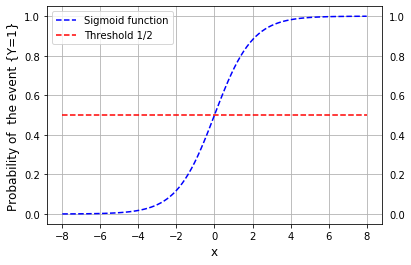
\includegraphics[width = .7\linewidth]{./Illustrations/logistic_function.png}
%\end{center}
%\caption{Logistic function $\sigma: x \mapsto \rme^x/(1+\rme^x)$.}
%\end{figure}
When $\alpha$ and $\beta$ are unknown, this classifier cannot be computed explicitely and is approximated using the observations. Assume that  $(X_i,Y_i)_{1\leqslant i\leqslant n}$ are independent observations with the same distribution as $(X,Y)$. The conditional  likelihood of the observations $Y_{1:n}$  given $X_{1:n}$ is:
\begin{align*}
\bP_{\theta}\left(Y_{1:n}\middle |X_{1:n}\right) &=\prod_{i=1}^n \bP_{\theta}\left(Y_{i} \middle |X_{i}\right)\eqsp,\\
&= \prod_{i=1}^n \left(\sigma_{\alpha,\beta}\right)^{(1+Y_i)/2}(X_i)\left(1-\sigma_{\alpha,\beta}(X_i)\right)^{(1-Y_i)/2}\eqsp,\\
&=  \prod_{i=1}^n \left(\frac{\rme^{\alpha + \langle \beta;X_i\rangle}}{1+\rme^{\alpha + \langle \beta;X_i\rangle}}\right)^{(1+Y_i)/2}\left( \frac{1}{1+\rme^{\alpha + \langle \beta;X_i\rangle}}\right)^{(1-Y_i)/2}\eqsp.
\end{align*}
The associated conditional loglikelihood is therefore
\begin{align*}
\log \bP_{\theta}\left(Y_{1:n}\middle |X_{1:n}\right) &=\sum_{i=1}^n \left\{\frac{1+Y_i}{2}\log\left(\frac{\rme^{\alpha + \langle \beta;X_i\rangle}}{1+\rme^{\alpha + \langle \beta;X_i\rangle}}\right) + \frac{1-Y_i}{2}\log\left(\frac{1}{1+\rme^{\alpha + \langle \beta;X_i\rangle}}\right) \right\}\eqsp,\\
&= \sum_{i=1}^n \left\{ \frac{1+Y_i}{2}\left(\alpha + \langle \beta;X_i\rangle\right) - \log\left(1+\rme^{\alpha + \langle \beta;X_i\rangle}\right)\right\}\eqsp.
\end{align*}
This conditional loglikelihood function cannot be maximized explictly yet numerous numerical optimization methods are available to maximize $(\alpha,\beta)\mapsto \log \bP_{\theta}\left(Y_{1:n}\middle |X_{1:n}\right)$. If $(\widehat \alpha_n,\widehat \beta_n)$ is an approximate solution to the optimization problem:
\begin{equation}
\label{eq:loglik:logistic}
(\widehat \alpha_n,\widehat \beta_n)\in \argmax_{\theta=(\alpha,\beta)\in\rset\times\rset^d}\log \bP_{\theta}(Y_{1:n}|X_{1:n})\eqsp,
\end{equation}
then the associated logistic regression classifier is given by
\[
\widehat h_{n}: x\mapsto  \left\{
    \begin{array}{ll}
       1 & \mbox{if }\; \widehat \alpha_n + \langle \widehat \beta_n;x\rangle>0\eqsp, \\
        -1 & \mbox{otherwise}\eqsp,
    \end{array}
\right.
\]
Even though, the model is semiparametric (and not parametric), it can be shown that, specifically for logistic regression model, the approximated classifier almost surely tends to the Bayes classifier as the number of observations $n$ tends to infinity.

\begin{figure}
\begin{center}
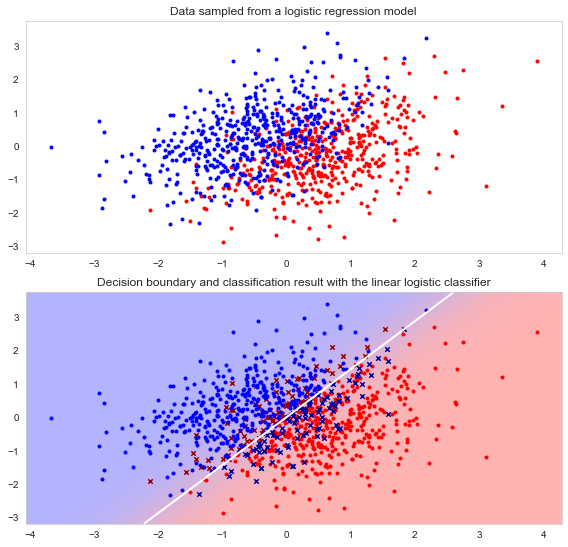
\includegraphics[width = .8\linewidth]{./Illustrations/logistic_decision.png}
\end{center}
\caption{(Top) Data are generated with a logistic regression model. The input data are Gaussian vectors in dimension $d = 2$ and the class of each data is chosen randomly according to \eqref{eq:prob:logistic} with a fixed weight $w$. (Bottom)  Classification boundary obtained with the logistic classifier. Crosses are all false positives i.e. all data wrongly classified by the classifier (eventhough the weight $w$ is known in this case). Simulations can be found here \url{https://sylvainlc.github.io/}.}
\end{figure}


Additional numerical considerations can be found for instance here \url{https://scikit-learn.org/stable/modules/linear\_model.html#logistic-regression}.


%The universal approximation theorem sets a theoretical guarentee that feedforward networks with hidden layers provide a universal approximation framework. The first result of (Horniket al., 1989; Cybenko, 1989) states that a feedforward network with a linear output layer and at least one hidden layer  can approximate any Borel measurable function from one finite-dimensional space to another, provided that the network is given enough hidden units. The derivatives of the feedforward network can also approximate the derivatives of the function arbitrarily well (Hornik et al., 1990). 
%\begin{theorem}[Horniket al., 1989; Cybenko, 1989]
%Let $\sigma$ be a bounded and continuous activation function. Then, for $p\geqslant 1$ and  all $f:\mathrm{L}^p(\mu,\rset^d,\rset)$ with $\mu$ a finite measure on $\rset^d$ and all $\varepsilon>0$ there exists $q\geqslant 1$ and parameter $\omega$, $\upsilon$ and $b$ such that writing
%\[
%\hat{f}_q :x \mapsto \sum_{i=1}^q\upsilon_i \sigma(\omega_i'x+b_i)
%\]
%yields
%\[
%\|f -\hat{f}_q\|_{p,\mu} \leqslant \varepsilon\eqsp.
%\]
%The neural networks with one hidden layer and a linear output are dense in $\mathrm{L}^p(\mu,\rset^d,\rset)$. When $\sigma$ is continuous, the neural networks with one hidden layer and a linear output are dense in $\mathcal{C}(K,\rset)$ for the topology of the supremum norm, where $K$ is a compact of $\rset^d$.
%\end{theorem}
%While the original theorems were first stated in terms of units with activation functions that saturate for both very negative and very positive arguments, universal approximation theorems have also been proved for a wider class of activation functions, which includes the now commonly used rectified linear unit (Leshno et al., 1993).
%\begin{theorem}[Leshno et al., 1993]
%Assume that $\sigma$ is not a polynomial activation function. Then, the neural networks associated with $\sigma$ is dense in $\mathcal{C}(\rset^d,\rset)$ for the topology of the supremum norm on compact subsets.
%\end{theorem}
%According to the universal approximation theorem, there exists a network largeenough to achieve any degree of accuracy we desire, but the theorem does notsay how large this network will be. Barron (1993) provides some bounds on thesize of a single-layer network needed to approximate a broad class of functions.Unfortunately, in the worst case, an exponential number of hidden units (possiblywith one hidden unit corresponding to each input configuration that needs to bedistinguished) may be required. 
%\begin{theorem}[Barron, 1993]
%Assume that $\sigma$ is not a polynomial activation function. Then, the exists a neural network associated with $\sigma$ such that
%\[
%\int_{\mathsf{B}(0,r)}\left(f(x) - \hat{f}_q(x)\right)^2\mu(\rmd x) \leqslant C\left(q^{-1} + \frac{qd}{n}\log n\right)\eqsp.
%\]
%\end{theorem}



%\subsection{Support vector machines} 
%\subsubsection*{Hard Support Vector Machines}
%Hard Support Vector Machines is a classification procedure which aims at  building a linear classifier with the largest possible margin, i.e. the largest minimal distance between a point in the training set and the hyperplane. The objective is to find a hyperplane which correclty separates all training data points by maximizing the closest distance from this hyperplane of a point in the training data set. Let $H_{w,b}$ be the hyperplane of $\rset^d$ with orthogonal vector $w$ and offset $b$:
%\[
%H_{w,b} = \{x\in\rset^d\eqsp;\eqsp \langle w\eqsp;\eqsp x\rangle + b = 0\}\eqsp.
%\]
%Following for instance the results obtained for linear discriminant analysis and logistic regression, a hyperplane $H_{w,b}$ may be used as a classifier by defining
%\[
%h_{w,b}: x \mapsto \left\{
%    \begin{array}{ll}
%       1 & \mbox{if }\;  \langle w\eqsp;\eqsp x\rangle + b >0\eqsp, \\
%        -1 & \mbox{otherwise}\eqsp.
%    \end{array}
%\right.
%\]
%Hard Support Vector Machines are applied in the case where the training data points are linearly separable which means that there exists a linear classifier $h_{w,b}$ with $(w,b)\in \rset^d\times \rset$, $\|w\| = 1$,  which classifies correctly all observed data, for all $1\leqslant i \leqslant n$,
%\[
%Y_i \left(\langle w\eqsp;\eqsp X_i\rangle + b\right) >0\eqsp.
%\]
%The distance between any $x\in\rset^d\setminus H_{w,b}$ and $H_{w,b}$ is given by
%\[
%d(x,H_{w,b}) = \left|\langle w\eqsp;\eqsp x\rangle + b\right|\eqsp.
%\]
%Therefore,  the hyperplane which correctly separates all training data sets with the largest margin is $H_{\widehat w_n,\widehat b_n}$ where
%\[
%(\widehat w_n,\widehat b_n)\in \underset{\substack{(w,b)\in\rset^d\times \rset^d\eqsp;\eqsp \|w\|=1,\\ \forall i\in\{1,\ldots,n\},\eqsp Y_i\left(\langle w\eqsp;\eqsp X_i\rangle + b\right) > 0}}{\argmax}\left\{\underset{1\leqslant i \leqslant n}{\min}\;\left|\langle w\eqsp;\eqsp X_i\rangle + b\right|\right\}\eqsp.
%\]
%\begin{shaded}
%\begin{proposition}
%The hard Support Vector Machines procedure is equivalent to solving the following optimization problem:
%\begin{equation}
%\label{eq:hardsvm}
%(\widehat w_n,\widehat b_n)\in \underset{(w,b)\in\rset^d\times \rset\eqsp;\eqsp \|w\|=1}{\argmax}\left\{\underset{1\leqslant i \leqslant n}{\min}\;Y_i\left(\langle w\eqsp;\eqsp X_i\rangle + b\right)\right\}\eqsp,
%\end{equation}
%\end{proposition}
%\end{shaded}
%\begin{proof}
%Let $(\widehat w_n,\widehat b_n)$ be a solution to \eqref{eq:hardsvm}. As the training data set is assumed to be linealry separable, there exist $(w,b)\in \rset^d\times \rset$ with $\|w\| = 1$ such that for all $1\leqslant i\leqslant n$, $Y_i(\langle w\eqsp;\eqsp X_i\rangle + b) > 0$. By definition of $(\widehat w_n,\widehat b_n)$ , 
%\[
%\underset{1\leqslant i \leqslant n}{\min}\;Y_i\left(\langle \widehat w_n\eqsp;\eqsp X_i\rangle + \widehat b_n\right) \geqslant \underset{1\leqslant i \leqslant n}{\min}\;Y_i\left(\langle w\eqsp;\eqsp X_i\rangle + b\right) >0
%\]
%and then $(\widehat w_n,\widehat b_n)$ satisfies the constraints of the hard Support Machines problem. On the other hand,  for any $(w,b)\in\rset^d\times \rset$ satisfying these constraints, for all $1\leqslant i \leqslant n$, $Y_i$ and $\langle w\eqsp;\eqsp X_i\rangle + b$ have the same sign, 
%\[
%\underset{1\leqslant i \leqslant n}{\min}\;Y_i\left(\langle w\eqsp;\eqsp X_i\rangle + b\right) = \underset{1\leqslant i \leqslant n}{\min}\;\left|\langle w\eqsp;\eqsp X_i\rangle + b\right|\eqsp,
%\]
%which concludes the proof.
%\end{proof}
%
%\begin{shaded}
%\begin{proposition}
%\label{prop:svm:quadratic}
%Define $(\widehat w_n,\widehat b_n) = (w_\star/\|w_\star\|,b_\star/\|w_\star\|)$ where
%\begin{equation}
%\label{eq:hardsvm:quadratic}
%(w_\star,b_\star)\in  \hspace{-.8cm}  \underset{\substack{(w,b)\in\rset^d\times \rset\\ \forall i\in\{1,\ldots,n\},\eqsp Y_i\left(\langle w\eqsp;\eqsp X_i\rangle + b\right)\geqslant 1}}{\argmin} \hspace{-.8cm} \|w\|^2\eqsp.
%\end{equation}
%Then, $(\widehat w_n,\widehat b_n)$ is a solution to \eqref{eq:hardsvm}.
%\end{proposition}
%\end{shaded}
%\begin{proof}
%Let $(w_\star,b_\star)$ be a solution to \eqref{eq:hardsvm:quadratic} and define  $(\widehat w_n,\widehat b_n) = (w_\star/\|w_\star\|,b_\star/\|w_\star\|)$. Therefore, $\|\widehat w_n\| = 1$ and 
%\[
%\underset{1\leqslant i \leqslant n}{\min}\;Y_i\left(\langle \widehat w_n\eqsp;\eqsp X_i\rangle + \widehat b_n\right)\geqslant \|w_\star\|^{-1}\eqsp.
%\]
%In addition, if $(w,b)\in\rset^d\times \rset$ is solution to \eqref{eq:hardsvm},
%\[
%\delta_{\star} = \underset{1\leqslant i \leqslant n}{\min}\;Y_i\left(\langle w\eqsp;\eqsp X_i\rangle + b\right)
%\]
%so that $(w/\delta_\star,b/\delta_\star)$ satisfies the constraints of \eqref{eq:hardsvm:quadratic} which yields $\|w_\star\|\leqslant \|w\|/\delta_\star\leqslant 1/\delta_\star$. Then, $\delta_\star \leqslant \|w_\star\|^{-1}$ which proves that $(\widehat w_n,\widehat b_n)$ is a solution to \eqref{eq:hardsvm}.
%\end{proof}
%The hard SVM problem displayed in Proposition~\ref{prop:svm:quadratic} is a convex quadratic problem with linear constraints. When the training dataset is assumed to be linearly separable, this problem has a unique solution which may be approximated efficiently using one of the numerous numerical optimization algorithms such as stochastic gradient procedures. On the other hand, the dual problem associated with  Proposition~\ref{prop:svm:quadratic} offers an alternative to obtain a solution to hard SVM. The Lagrangian function associated with this problem is
%\[
%\mathcal{L}: (w,b,\mu) \mapsto \|w\|^2+ \sum_{i=1}^n \mu_i\left(1 - Y_i\left(\langle w\eqsp;\eqsp X_i\rangle + b\right)\right)
%\]
%and the Lagrangian dual problem is 
%\[
%\widehat \mu \in \underset{\mu_i \geqslant 0}{\argmax}\;  \left\{\inf_{(w,b)\in\rset^d\times  \rset} \mathcal{L}(w,b,\mu)\right\} \eqsp.
%\]
%As the function to be minimized is convex and  continuously differentiable and the inequality constraints are affine, $(\widehat w, \widehat b)\in\rset^{d+1}$ is  solution to \eqref{prop:svm:quadratic} if and only if there exists $\mu\in\rset^{d}$ such that, for all $1\leqslant i \leqslant n$, $\partial_{w_i}\mathcal{L}(\widehat w,\widehat b,\mu) = 0$,  $\partial_{b}\mathcal{L}(\widehat w,\widehat b,\mu) = 0$, $Y_i(\langle \widehat w\eqsp;\eqsp X_i\rangle + \widehat b)\leqslant 1$, $\mu_i\geqslant 0$, and  $\mu_i(Y_i(\langle \widehat w\eqsp;\eqsp X_i\rangle + \widehat b)-1) = 0$. This yields 
%\[
%\widehat w = 2^{-1}\sum_{i=1}^n \mu_i Y_iX_i\quad\mathrm{and} \quad\sum_{i=1}^n\mu_i Y_i = 0\eqsp.
%\]
%For all $1\leqslant i \leqslant n$, if $Y_i(\langle \widehat w\eqsp;\eqsp X_i\rangle + \widehat b) > 1$ and then $\mu_i = 0$ and the $i$-th observation is not involved in $\widehat w$. Conversely, if $\mu_i>0$, then $|\langle \widehat w\eqsp;\eqsp X_i\rangle + \widehat b| = 1$, the margin of all observations involved in $\widehat w$ is $1$. These vectors are called the {\em support vectors}. Note that $\mu$ is solution to the dual problem
%\[
%\mu  \in \underset{\substack{\mu_i \geqslant 0\\ \sum_{i=1}^n\mu_i Y_i = 0}}{\argmax}\; \left\{\sum_{i=1}^n\mu_i - \frac{1}{2}\sum_{1\leqslant i,j\leqslant n}\mu_i\mu_j Y_iY_j \langle X_i\eqsp;\eqsp X_j\rangle\right\}\eqsp.
%\]
%
%
%\begin{figure}
%\begin{center}
%\includegraphics[scale = .5]{./Data/linear_svm_data.png}
%\includegraphics[scale = .5]{./Data/linear_svm_classifier.png}
%\includegraphics[scale = .5]{./Data/linear_svm_support_vectors.png}
%\end{center}
%\caption{(Top left) Linearly separable dataset, as shown by a hyperplane which separactes correctly both classes  and (top right) hard SVM classifier and its margin (solid line). (Bottom) hard SVM classifier with its  three support vectors (black dots). These support vectors are those such that $\mu_i>0$ and  then $\langle \widehat w\eqsp;\eqsp X_i\rangle + \widehat b \in\{-1\eqsp;\eqsp 1\}$. They are on the contour lines with level $1$ or $-1$ of the function $x \mapsto \langle \widehat w\eqsp;\eqsp x\rangle + \widehat b$ (dashed lines).}
%\end{figure}
%
%\subsubsection*{Soft Support Vector Machines}
%By Proposition~\ref{prop:svm:quadratic}, the hard Support Vector Machines can be reduced to a  quadratic optimization problem with linear constraints,  which may be solved in a reasonable computational time, when the training data sets is linearly separable.  Restricting the problem to linearly separable  training data sets is a somehow strong assumption. Soft Support Vector Machines algorithm introduces a relaxation of this constraint which can be applied with nonlinearly separable data sets. In this setting, the inequality constraints in the quadratic optimization problem \eqref{eq:hardsvm:quadratic} can be relaxed by introducing nonnegative variables $(\xi_i)_{1\leqslant i \leqslant n}$ which quantify for each variable $1\leqslant i \leqslant n$, the nonfeasability of the constraint $Y_i(\langle w\eqsp;\eqsp X_i\rangle + b)\geqslant 1$. Therefore, the soft Support Vector Machines algorithm simultaneously the margin of the linear classifier and the average value of these slack variables $(\xi_i)_{1\leqslant i \leqslant n}$:
%\begin{equation}
%\label{eq:softsvm:withslack}
%(w_\star,b_\star,\xi_\star)\in  \hspace{-.8cm}  \underset{\substack{(w,b,\xi)\in\rset^d\times \rset\times\rset_+^d\\ \forall i\in\{1,\ldots,n\},\eqsp Y_i\left(\langle w\eqsp;\eqsp X_i\rangle + b\right)\geqslant 1-\xi_i}}{\argmin} \hspace{-.5cm} \left\{\lambda\|w\|^2 + \frac{1}{n}\sum_{i=1}^n\xi_i\right\}\eqsp,
%\end{equation}
%where $\lambda >0$. 
%
%\begin{remark}
%In this case, for all $1\leqslant i \leqslant n$, if $Y_i\left(\langle w\eqsp;\eqsp X_i\rangle + b\right)\geqslant 1$, then $\xi_{\star,i} = 0$ and if $Y_i(\langle w\eqsp;\eqsp X_i\rangle + b)<1$ then the optimal choice for $\xi_{\star,i}$ is $\xi_{\star,i} = 1-Y_i(\langle w\eqsp;\eqsp X_i\rangle + b)$. Therefore, for all $1\leqslant i\leqslant n$,
%\[
%\xi_{\star,i} = \left(1-Y_i(\langle w\eqsp;\eqsp X_i\rangle + b)\right)_+\eqsp.
%\]
%Conversely, if $(w_\star,b_\star)$ is solution to
%\begin{equation}
%\label{eq:softsvm:withoutslack}
%(w_\star,b_\star)\in  \underset{(w,b)\in\rset^d\times \rset}{\argmin}  \left\{\lambda\|w\|^2 + \frac{1}{n}\sum_{i=1}^n(1-Y_i\left(\langle w\eqsp;\eqsp X_i\rangle + b\right))_+\right\}\eqsp,
%\end{equation}
%then $(w_\star,b_\star,\xi_\star)$ is solution to \eqref{eq:softsvm:withslack} with for all $1\leqslant i \leqslant n$, $\xi_{\star,i} = (1-Y_i\left(\langle w\eqsp;\eqsp X_i\rangle + b\right))_+$. Therefore, the linear classifier produced by the soft Support Vector Machines is solution to \eqref{eq:softsvm:withoutslack}. This formulation of the Soft SVM problem motivates the introduction of kernel based SVM detailed at the end of this chapter.
%\end{remark}
%
%The optimization problem \eqref{eq:softsvm:withslack} can be written 
%\begin{equation}
%\label{eq:optimization:svm:smooth:kkt}
%(\widehat w, \widehat \xi,\widehat b) \in \underset{\substack{h_i(\xi,w,b)\leqslant 0\eqsp,\\ g_i(\xi,w,b)\leqslant 0}}{\argmin}\; f(\xi,w,b) \eqsp,
%\end{equation}
%where $f:(\xi,w,b) \to\ n^{-1}\sum_{i=1}^n \xi_i + \lambda \|w\|^2$ and for all $1\leqslant i \leqslant n$, $g_i:(\xi,w,b) \mapsto -\xi_i $ and $h_i:(\xi,w,b) \mapsto 1 - \xi_i -Y_i(\langle w\eqsp;\eqsp X_i\rangle + b)$. The Lagrangian function associated with this problem is
%\[
%\mathcal{L}: (\xi,w,b,\mu,\gamma) \mapsto f(\xi,w,b) + \sum_{i=1}^n \mu_ih_i(\xi,w,b) + \sum_{i=1}^n \gamma_ig_i(\xi,w,b)
%\]
%and the Lagrangian dual problem is 
%\[
%(\widehat \mu,\widehat \gamma) \in \underset{\mu_i \geqslant 0\eqsp,\eqsp \gamma_i\geqslant 0}{\argmax}\;  \left\{\inf_{(\xi,w,b)\in\rset^d\times \rset^d\times  \rset} \mathcal{L}(\xi,w,b,\mu,\gamma)\right\} \eqsp.
%\]
%As the function to be minimized is convex and  continuously differentiable and the inequality constraints are affine, $(\widehat w, \widehat \xi,\widehat b)\in\rset^{2d+1}$ is  solution to \eqref{eq:optimization:svm:smooth:kkt} if and only if there exists $(\mu,\gamma)\in\rset^{2d}$ such that, for all $1\leqslant i \leqslant n$, $\partial_{\xi_i}\mathcal{L}(\widehat \xi,\widehat w,\widehat b,\mu,\gamma) = 0$,  $\partial_{w_i}\mathcal{L}(\widehat \xi,\widehat w,\widehat b,\mu,\gamma) = 0$ and $\partial_{b}\mathcal{L}(\widehat \xi,\widehat w,\widehat b,\mu,\gamma) = 0$, $h_i(\widehat \xi,\widehat w,\widehat b)\leqslant 0$,  $g_i(\widehat \xi,\widehat w,\widehat b)\leqslant 0$, $\mu_i\geqslant 0$, $\gamma_i\geqslant 0$,  $\mu_ig_i(\widehat \xi,\widehat w,\widehat b) = 0$ and  $\gamma_i h_i(\widehat \xi,\widehat w,\widehat b) =  0$. This yields 
%\[
%w = (2\lambda)^{-1}\sum_{i=1}^n \mu_i Y_iX_i\eqsp,\quad \mu_i + \gamma_i = 1/n \quad\mathrm{and} \quad\sum_{i=1}^n\mu_i Y_i = 0\eqsp.
%\]
%Then $w = (2\lambda)^{-1}\sum_{i=1}^n \mu_i Y_iX_i$ and $\mu$ is solution to
%\[
%\mu  \in \underset{\substack{0 \leqslant \mu_i \leqslant 1/n\\ \sum_{i=1}^n\mu_i Y_i = 0}}{\argmax}\; \left\{\sum_{i=1}^n\mu_i - \frac{1}{2\lambda}\sum_{1\leqslant i,j\leqslant n}\mu_i\mu_j Y_iY_j \langle X_i\eqsp;\eqsp X_j\rangle\right\}\eqsp.
%\]
%Therefore, the normal vector of the hyperplane is a linear combination of the $(X_i)_{1\leqslant i\leqslant n}$ where $\mu$ is solution to a quadratic optimization problem which only involves $(X_i)_{1\leqslant i\leqslant n}$ through $( \langle X_i\eqsp;\eqsp X_j\rangle)_{1\leqslant i,j\leqslant n}$.
%
%\begin{figure}
%\begin{center}
%\includegraphics[scale = .5]{./Data/soft_svm_smallC.png}
%\includegraphics[scale = .5]{./Data/soft_svm_largeC.png}
%\end{center}
%\caption{(Left) Soft SVM classifier (solid line) and support vectors (black dots) for a chosen $\lambda_0$. (Right) soft SVM classifier with its  with $\lambda = 100 \lambda_0$. The support vectors are those such that $\mu_i>0$ and  then $|\langle \widehat w\eqsp;\eqsp X_i\rangle + \widehat b |<1 $. They are inbetween the contour lines with level $1$ or $-1$ of the function $x \mapsto \langle \widehat w\eqsp;\eqsp x\rangle + \widehat b$ (dashed lines).}
%\end{figure}
%
%

\section{Nonparametric Bayes classifier}
\index{models!nonparametric}
In the case of {\em nonparametric} models, it is not assumed anymore that the joint law of $(X,Y)$ belongs to any parametric or semiparametric family of models. The assumption on the distribution of $(X,Y)$ is relaxed but instead, we will make some restrictions on the set of classifiers on which the optimisation occurs.

%Another approach which allows to weaken the assumptions on the joint distribution of $(X,Y)$ is to 
More precisely, we consider that the optimization of classifiers holds on a specific set $\calH$ of classifiers (often called the {\em dictionary}\index{dictionary}), which may possibly not contain the Bayes classifier. Moreover, since in most cases, the classification risk $\Lmiss$ cannot be computed nor  minimized, it is instead estimated by the empirical classification risk \index{classification risk!empirical} defined as
\[
\widehat {\mathsf{R}}^n_{\mathrm{miss}}(h) = \frac{1}{n}\sum_{i=1}^n \1_{Y_i \neq h(X_i)}\eqsp,
\]
where  $(X_i,Y_i)_{1\leqslant i\leqslant n}$ are independent observations with the same distribution as $(X,Y)$. The classification problem then boilds down to solving
\begin{equation}
\label{eq:empirical:classif}
\widehat h^n_{\calH} \in \underset{h\in\calH}{\argmin}\;\widehat {\mathsf{R}}^n_{\mathrm{miss}}(h)\eqsp.
\end{equation}
In this context several practical and theoretical challenges arise from the minimization of the empirical classification risk. The choice of $\calH$ is pivotal in designing an efficient classification procedure. Note that choosing $\calH$ as all possible classifiers is meaningless, in this case, $\widehat h^n_{\calH}$ is such that $\widehat h^n_{\calH}(X_i) = Y_i$ for all $1 \leqslant i\leqslant n$ and $\widehat h^n_{\calH}(x)$ is any element of $\{-1,1\}$ for all $x\notin\{X_1,\ldots,X_n\}$. Although $\widehat{\mathsf{R}}^n_{\mathrm{miss}}(h^n_{\calH}) = 0$,  is likely to be  a poor approximation of $\mathsf{R}_{\mathrm{miss}}(h^n_{\calH})$. To understand this, the excess misclassification risk may be decomposed as follows
\[
\mathsf{R}_{\mathrm{miss}}\left(\widehat h^n_{\calH}\right) - \mathsf{R}_{\mathrm{miss}}\left(h_{\star}\right) = \mathsf{R}_{\mathrm{miss}}\left(\widehat h^n_{\calH}\right) - \underset{h\in\calH}{\min}\; \mathsf{R}_{\mathrm{miss}}\left(h\right)  + \underset{h\in\calH}{\min}\; \mathsf{R}_{\mathrm{miss}}\left(h\right)  -  \mathsf{R}_{\mathrm{miss}}\left(h_{\star}\right) \geqslant 0\eqsp.
\]
The first term of the decomposition $\mathsf{R}_{\mathrm{miss}}(\widehat h^n_{\calH}) - \min_{h\in\calH}\; \mathsf{R}_{\mathrm{miss}}\left(h\right)$ is a \textbf{stochastic error} which is likely to grow when the size of $\calH$ grows while $\min_{h\in\calH}\; \mathsf{R}_{\mathrm{miss}}\left(h\right)  -  \mathsf{R}_{\mathrm{miss}}\left(h_{\star}\right)$ is \textbf{deterministic} and likely to decrease as the size of $\calH$ grows.
%\rd{J ai pas compris pourquoi cette erreur stochastique devrait augmenter avec la taille du dictionary}
\begin{shaded}
\begin{lemma}
\label{lem:missclassif:ub}
For all set $\calH$ of classifiers and all $n\geqslant 1$,
\begin{equation}
\label{eq:stochError}
\mathsf{R}_{\mathrm{miss}}(\widehat h^n_{\calH}) - \underset{h\in\calH}{\min}\; \mathsf{R}_{\mathrm{miss}}\left(h\right) \leqslant 2 \underset{h\in\calH}{\sup}\left|\widehat{\mathsf{R}}^n_{\mathrm{miss}}(h) - \mathsf{R}_{\mathrm{miss}}\left(h\right)\right| \eqsp.
\end{equation}
\end{lemma}
\end{shaded}
\begin{proof}
By definition of $\widehat h^n_{\calH}$, for any $h\in\calH$,
\begin{align*}
\mathsf{R}_{\mathrm{miss}}(\widehat h^n_{\calH}) - \underset{h\in\calH}{\min}\; \mathsf{R}_{\mathrm{miss}}\left(h\right) &=  \mathsf{R}_{\mathrm{miss}}(\widehat h^n_{\calH})  - \widehat {\mathsf{R}}^n_{\mathrm{miss}}(\widehat h^n_{\calH}) + \widehat {\mathsf{R}}^n_{\mathrm{miss}}(\widehat h^n_{\calH}) - \underset{h\in\calH}{\min}\; \mathsf{R}_{\mathrm{miss}}\left(h\right)\eqsp,\\
&\leqslant \mathsf{R}_{\mathrm{miss}}(\widehat h^n_{\calH})  - \widehat {\mathsf{R}}^n_{\mathrm{miss}}(\widehat h^n_{\calH}) + \widehat {\mathsf{R}}^n_{\mathrm{miss}}(h) - \underset{h\in\calH}{\min}\; \mathsf{R}_{\mathrm{miss}}\left(h\right)\eqsp.
\end{align*}
For all $\varepsilon>0$ there exists $h_{\varepsilon}\in\calH$ such that  $\mathsf{R}_{\mathrm{miss}}(h_{\varepsilon})< \min_{h\in\calH}\; \mathsf{R}_{\mathrm{miss}}\left(h\right) + \varepsilon$ so that
\begin{align*}
\mathsf{R}_{\mathrm{miss}}(\widehat h^n_{\calH}) - \underset{h\in\calH}{\min}\; \mathsf{R}_{\mathrm{miss}}\left(h\right) &\leqslant \mathsf{R}_{\mathrm{miss}}(\widehat h^n_{\calH})  - \widehat {\mathsf{R}}^n_{\mathrm{miss}}(\widehat h^n_{\calH}) + \widehat {\mathsf{R}}^n_{\mathrm{miss}}(h_{\varepsilon}) - \mathsf{R}_{\mathrm{miss}}(h_{\varepsilon}) + \varepsilon\eqsp,\\
&\leqslant   2 \underset{h\in\calH}{\sup}\left|\widehat {\mathsf{R}}^n_{\mathrm{miss}}(h) - \mathsf{R}_{\mathrm{miss}}\left(h\right)\right| + \varepsilon\eqsp,
\end{align*}
which concludes the proof.
\end{proof}

\subsection*{Oracle inequality when $\calH$ is finite}
This section considers the simple case where the dictionary is finite, i.e., $\calH = \{h_1,\ldots,h_M\}$ where $M\geqslant 1$ and for all $1\leqslant j\leqslant M$, $h_j:\xset \to\{-1,1\}$ is a given classifier.
%Let $h_{\calH}$ be such as
%\[
%L_{\mathrm{miss}}(h_{\calH}) = \underset{1\leqslant j \leqslant M}{\min}L_{\mathrm{miss}}(h_j)\eqsp.
%\]

\begin{shaded}
\begin{proposition}
\label{prop:oracle:finite:prob}
Assume that  $\calH = \{h_1,\ldots,h_M\}$, then, for all $\delta>0$,
\[
\bP\left(\mathsf{R}_{\mathrm{miss}}(\widehat h^n_{\calH}) \leqslant \underset{1\leqslant j \leqslant M}{\min}\mathsf{R}_{\mathrm{miss}}(h_j) + \sqrt{\frac{2}{n}\log\left(\frac{2M}{\delta}\right)}\right)\geqslant 1-\delta\eqsp.
\]
\end{proposition}
\end{shaded}
\begin{proof}
By \Cref{lem:missclassif:ub}, for all $u>0$,
\[
\bP\left(\mathsf{R}_{\mathrm{miss}}(\widehat h^n_{\calH}) > \underset{1\leqslant j \leqslant M}{\min}\mathsf{R}_{\mathrm{miss}}(h_j) + u\right) \leqslant \bP\left( \underset{h\in\calH}{\sup}\left|\widehat {\mathsf{R}}^n_{\mathrm{miss}}(h) - \mathsf{R}_{\mathrm{miss}}\left(h\right)\right|  > \frac{u}{2}\right) \leqslant \sum_{j=1}^M  \bP\left(\left|\widehat {\mathsf{R}}^n_{\mathrm{miss}}(h_j) - \mathsf{R}_{\mathrm{miss}}\left(h_j\right)\right|  > \frac{u}{2}\right)\eqsp.
\]
By Hoeffding's inequality, see Theorem~\ref{th:hoeffding},
\[
\bP\left(\mathsf{R}_{\mathrm{miss}}(\widehat h^n_{\calH}) > \underset{1\leqslant j \leqslant M}{\min}\mathsf{R}_{\mathrm{miss}}(h_j) + u\right) \leqslant 2M\rme^{-nu^2/2}\eqsp,
\]
which concludes the proof by choosing
\[
u = \sqrt{\frac{2}{n}\log\left(\frac{2M}{\delta}\right)}\eqsp.
\]
\end{proof}

\begin{shaded}
\begin{proposition}
\label{prop:oracle:finite:expectation}
Assume that  $\calH = \{h_1,\ldots,h_M\}$, then,
\[
\bE\left[\mathsf{R}_{\mathrm{miss}}(\widehat h^n_{\calH})\right] \leqslant \underset{1\leqslant j \leqslant M}{\min}\mathsf{R}_{\mathrm{miss}}(h_j) + \sqrt{\frac{2\log\left(2M\right)}{n}}\eqsp.
\]
\end{proposition}
\end{shaded}



\begin{proof}
By \Cref{lem:missclassif:ub},
$$
\bE\left[\mathsf{R}_{\mathrm{miss}}(\widehat h^n_{\calH})\right]  - \underset{1\leqslant j \leqslant M}{\min}\mathsf{R}_{\mathrm{miss}}(h_j) \leqslant  2 \bE\left[\underset{h\in\calH}{\sup}\left|\widehat {\mathsf{R}}^n_{\mathrm{miss}}(h) - \mathsf{R}_{\mathrm{miss}}\left(h\right)\right|  \right]=\frac{2 }{n} \bE\left[ \underset{1\leqslant j\leqslant M}{\max}\left\{n\left|\widehat {\mathsf{R}}^n_{\mathrm{miss}}(h_j) - \mathsf{R}_{\mathrm{miss}}\left(h_j\right)\right| \right\}\right]\eqsp.
$$
Note that
\[
n\left\{\widehat {\mathsf{R}}^n_{\mathrm{miss}}(h_j) -  \mathsf{R}_{\mathrm{miss}}\left(h_j\right)\right\} = \sum_{i=1}^n \left\{\1_{Y_i \neq h_j(X_i)}  -  \mathsf{R}_{\mathrm{miss}}\left(h_j\right)\right\}\eqsp,
\]
where the random variables $(\1_{Y_i \neq h_j(X_i)})_{1\leqslant i \leqslant n}$ are independent Bernoulli random variables with mean $\mathsf{R}_{\mathrm{miss}}(h_j)$. By Lemma~\ref{lem:bernoulli:bound}, for all $t>0$,
\[
\bE\left[\mathrm{exp}\left\{t\sum_{i=1}^n \left\{\1_{Y_i \neq h_j(X_i)}  -  \mathsf{R}_{\mathrm{miss}}\left(h_j\right)\right\}\right\}\right] = \prod_{i=1}^n \bE\left[\mathrm{exp}\left\{t\left(\1_{Y_i \neq h_j(X_i)}  -  \mathsf{R}_{\mathrm{miss}}\left(h_j\right)\right)\right\}\right] \leqslant \rme^{nt^2/8}
\]
and similarly
\[
\bE\left[\mathrm{exp}\left\{-t\sum_{i=1}^n \left\{\1_{Y_i \neq h_j(X_i)}  -  \mathsf{R}_{\mathrm{miss}}\left(h_j\right)\right\}\right\}\right] \leqslant \rme^{nt^2/8}\eqsp.
\]
Then, for all $t>0$, by Jensen's inequality,
\begin{align*}
\mathrm{exp}\left\{t \bE\left[ \underset{1\leqslant j\leqslant M}{\max}\left\{n\left|\widehat {\mathsf{R}}^n_{\mathrm{miss}}(h_j) - \mathsf{R}_{\mathrm{miss}}\left(h_j\right)\right| \right\}\right]\right\} &\leqslant \bE\left[\mathrm{exp}\left\{t\underset{1\leqslant j\leqslant M}{\max}\left\{n\left|\widehat {\mathsf{R}}^n_{\mathrm{miss}}(h_j) - \mathsf{R}_{\mathrm{miss}}\left(h_j\right)\right|\right\}\right\}\right] \eqsp,\\
%&\leqslant \sum_{j=1}^M  \bE\left[\mathrm{exp}\left\{t\left\{n\left(\widehat L^n_{\mathrm{miss}}(h_j) - L_{\mathrm{miss}}\left(h_j\right)\right)\right\}\right\}\right]\eqsp,\\
&\leqslant 2M\rme^{nt^2/8}\eqsp,
\end{align*}
which yields
\[
 \bE\left[ \underset{1\leqslant j\leqslant M}{\max}\left\{n\left|\widehat {\mathsf{R}}^n_{\mathrm{miss}}(h_j) - \mathsf{R}_{\mathrm{miss}}\left(h_j\right)\right| \right\}\right] \leqslant \frac{\log (2M)}{t} + \frac{nt}{8}\eqsp.
\]
Choosing $t= \sqrt{8\log (2M)/n}$,
\[
 \bE\left[ \underset{1\leqslant j\leqslant M}{\max}\left\{n\left|\widehat {\mathsf{R}}^n_{\mathrm{miss}}(h_j) - \mathsf{R}_{\mathrm{miss}}\left(h_j\right)\right|\right\}\right] \leqslant \sqrt{n\log(2M)/2}\eqsp,
\]
which concludes the proof.
\end{proof}











%
%\section{Classification based on convexification}
%
%Nonparametric classification based on the empirical risk minimization may seem appealing  
%since its statistical properties, such as oracle inequalities, can be obtained simply. However, these properties cannot be used to
%derive efficient practical classifiers due to the computational cost of the optimization problem defined by \eqref{eq:empirical:classif}. One of the most popular approach to design efficient algorithm for classification follows from a convexification of the original problem \eqref{eq:empirical:classif}.  The target loss function $\widehat L^n_{\mathrm{miss}}$ is replaced by a convex surrogate and its minimization is constrained to a convex set of classifiers.
%
%For any convex function $f:\xset\to \rset$, it is possible to build a classifier $h$ given by $h_f=\mathrm{sign}(f)$. The associated empirical classification is then
%\[
%\widehat L^n_{\mathrm{miss}}(h_f) = \frac{1}{n}\sum_{i=1}^n \1_{Y_i \neq h_f(X_i)} = \frac{1}{n}\sum_{i=1}^n \1_{Y_if(X_i) <0}\eqsp.
%\]
%Then, replacing the indicator function by any convex loss funtion $\ell$ yields a convex surrogate of $\widehat L^n_{\mathrm{miss}}$:
%\[
%\widehat L^{n,\mathrm{conv}}_{\mathrm{miss}}(f) = \frac{1}{n}\sum_{i=1}^n \ell(Y_if(X_i))\eqsp.
%\]
%Assume then that $\calF$ is a convex set of functions from $\xset$ to $\rset$. An approximate classifier can be efficiently computed by solving the following optimization problem.
%\begin{equation}
%\label{eq:empirical:classif:conv}
%\widehat f^n_{\calF} \in \underset{f\in\calF}{\argmin}\;\widehat L^{n,\mathrm{conv}}_{\mathrm{miss}}(f)\eqsp.
%\end{equation}
%In addition, when the smoothness of the function $f$ is penalized, $\widehat L^{n,\mathrm{conv}}_{\mathrm{miss}}$ may be  replaced by 
%\begin{equation}
%\label{eq:erm:rkhs}
%\widehat L^{n,\mathrm{conv}}_{\mathrm{miss}}(f) = \frac{1}{n}\sum_{i=1}^n \ell(Y_if(X_i)) + \lambda\|f\|^2\eqsp,
%\end{equation}
%where $\lambda>0$ and $\|\cdot\|$ is a norm on the space $\calF$. The soft Support Vector Machines algorithm defined by \eqref{eq:softsvm:withoutslack} fits this framework with the affine base function $f:x\mapsto \langle w\eqsp;\eqsp x\rangle + b$ and $\ell$ chosen as the hinge loss $\ell: x \mapsto (1-x)_+$ when the target function is penalized by its margin $\|w\|^2$.
%
%
%
%
%A useful case in practice consists in choosing $\calF$ as a Reproducing Kernel Hilbert Space with positive definite reproducing kernel $k$ on $\xset\times \xset$.
%
%\begin{shaded}
%\begin{definition}
%\label{def:kernel}
%A function $k:\xset\times\xset:\to \rset$ is said to be a positive semi-definite kernel if and only if it is symmetric and if for all $n\geqslant 1$, $(x_1,\ldots,x_n)\in\xset^n$ and all $(a_1,\ldots,a_n)\in\rset^n$,
%\[
%\sum_{1\leqslant i,j\leqslant n}a_ia_jk(x_i,x_j) \geqslant 0\eqsp.
%\]
%\end{definition}
%\end{shaded}
%
%\begin{remark}
%The following functions, defined on $\rset^d\times\rset^d$, are positive semi-definite kernels:
%$$
%k:(x,y)\mapsto x^Ty \quad\mathrm{and}\quad k:(x,y)\mapsto \mathrm{exp}\left(-\|x-y\|^2/(2\sigma^2\right)\eqsp,\; \sigma>0\eqsp.
%$$
%\end{remark}
%
%\begin{shaded}
%\begin{definition}
%Let $\calF$ be a Hilbert space of functions $f:\xset\to\rset$. A symmetric function $k:\xset\times\xset:\to \rset$ is said to be a reproducing kernel of $\calF$ if and only if for all $x\in\xset$, $k(x,\cdot)\in\calF$ and for all $x\in\Xset$ and all $f\in\calF$, $\langle f; k(x,\cdot)\rangle = f(x)$. The space $\calF$ is said to be a reproducing kernel Hilbert space with kernel $k$.
%\end{definition}
%\end{shaded}
%A reproducing kernel associated with a reproducing kernel Hilbert space is positive semi-definite since for all $n\geqslant 1$, $(x_1,\ldots,x_n)\in\xset^n$ and all $(a_1,\ldots,a_n)\in\rset^n$,
%\[
%\sum_{1\leqslant i,j\leqslant n}a_ia_jk(x_i,x_j) = \sum_{1\leqslant i,j\leqslant n}a_ia_j \langle k(x_i,\cdot);k(x_j,\cdot)\rangle = \left\|\sum_{1\leqslant i\leqslant n}a_i\langle k(x_i,\cdot)\right\|^2 \geqslant 0\eqsp.
%\]
%
%\begin{remark}
%The positive semi-definite kernel $k:(x,y)\mapsto x^Ty$ defined on $\rset^d\times\rset^d$ is a reproducing kernel of the space
%$$
%\calF = \left\{f: \rset^d\to\rset\eqsp;\eqsp \exists \omega\in\rset^d \eqsp\forall x\in \rset^d\eqsp, \eqsp f(x) = \omega^Tx\right\}\eqsp,
%$$
%equipped with the inner product defined, for all $(f,g)\in\calF\times\calF$, by 
%$$
%\langle f; g\rangle = \omega_f^T\omega_g\eqsp, 
%$$
%where $\omega_f,\omega_g\in\rset^d$ and $f: x\mapsto \omega_f^Tx$, $g: x\mapsto \omega_g^Tx$. 
%\end{remark}
%
%%\begin{shaded}
%%\begin{definition}
%%\label{def:rkhs}
%%Let $k:\xset\times\xset:\to \rset$ be a positive semi-definite kernel. The Reproducing Kernel Hilbert Space with kernel $k$ is the only Hilbert space $\calF \subset \rset^\Xset$ such that for all $x\in\xset$,  $k(x,\cdot) \in \calF$ and for all $x\in\Xset$ and all $f\in\calF$,
%%\[
%%f(x) = \langle f\eqsp;\eqsp k(x,\cdot)\rangle_\calF\eqsp.
%%\]
%%\end{definition}
%%\end{shaded}
%Proposition~\ref{prop:minimization:rkhs} proves that the minimization of the penalized empirical loss amounts to solving a convex optimization problem on $\rset^n$ for which many efficient  numerical solution exist.
%\begin{shaded}
%\begin{proposition}
%\label{prop:minimization:rkhs}
%Let $k:\xset\times\xset:\to \rset$ be a positive definite kernel and $\calF$ the RKHS with kernel $k$. Then, 
%\[
%\widehat f^n_{\calF} \in \underset{f\in\calF}{\argmin}\;\frac{1}{n}\sum_{i=1}^n \ell(Y_if(X_i)) + \lambda\|f\|_\calF^2\eqsp,
%\]
%where $\|f\|^2_\calF = \langle f\eqsp;\eqsp f\rangle$, is given by $\widehat f^n_{\calF} : x \mapsto \sum_{i=1}^n \widehat \alpha_i k(X_i,x)$, where
%\[
%\widehat\alpha \in \underset{\alpha \in \rset^n}{\argmin}\;\left\{\frac{1}{n}\sum_{i=1}^n \ell\left(\sum_{j=1}^n\alpha_jY_ik(X_j,X_i)\right) + \lambda \sum_{1\leqslant i,j \leqslant n}\alpha_i \alpha_j k(X_i,X_j)\right\}\eqsp.
%\]
%\end{proposition}
%\end{shaded}
%\begin{proof}
%Let $V$ be the linear space spanned by $(k(X_i,\cdot))_{1\leqslant i\leqslant n}$. For all $f\in\calF$, $f$ can be written $f = f_V + f_{V^\perp}$ with $f_V\in V$ and $f_{V^\perp}\in V^\perp$. Since $\calF$ is a RKHS with kernel $k$, for all $1\leqslant i \leqslant n$,
%\[
%f_{V^\perp}(X_i) = 0\quad \mathrm{and} \quad f(X_i) = \langle f\eqsp;\eqsp k(X_i,\cdot)\rangle = f_V(X_i)\eqsp.
%\]
%Therefore,
%\[
%\frac{1}{n}\sum_{i=1}^n \ell(Y_if(X_i)) + \lambda\|f\|^2 = \frac{1}{n}\sum_{i=1}^n \ell(Y_if_V(X_i)) + \lambda\|f_V\|^2 + \lambda\|f_{V^\perp}\|^2
%\]
%and any minimizer of the target function is in $V$. There exist $(\alpha_1,\ldots,\alpha_n)\in \rset^n$ such that 
%\[
%\widehat f^n_{\calF} :x\mapsto \sum_{i=1}^n \alpha_i k(X_i,x)\eqsp,
%\]
%which concludes the proof.
%\end{proof}
%In the special case of the soft Support Vector Machines, the solution to the convex problem is $\widehat f^n_{\calF}: x \mapsto   \sum_{i=1}^n \widehat \alpha_i k(X_i,x)$ where
%\[
%\widehat \alpha \in \underset{f\in\calF}{\argmin}\;\frac{1}{n}\sum_{i=1}^n (1-Y_if(X_i))_+ + \lambda \alpha^TK\alpha\eqsp,
%\]
%\begin{shaded}
%\begin{proposition}
%\label{prop:svm}
%Let $k:\xset\times\xset:\to \rset$ be a positive definite kernel and $\calF$ the RKHS with kernel $k$. Then, a solution to
%\[
%\widehat f^n_{\calF} \in \underset{f\in\calF}{\argmin}\;\frac{1}{n}\sum_{i=1}^n (1-Y_if(X_i))_+ + \lambda\|f\|^2\eqsp,
%\]
%is given by $\widehat f^n_{\calF}: x \mapsto   \sum_{i=1}^n \widehat \alpha_i k(X_i,x)$, where, for all $1\leqslant i\leqslant n$,
%\begin{align*}
%\widehat \alpha_i &= 0  \quad \mathrm{if} \quad Y_i\widehat f^n_{\calF}(X_i)>1\eqsp,\\
%\widehat \alpha_i &= Y_i/(2\lambda n)  \quad \mathrm{if} \quad Y_i\widehat f^n_{\calF}(X_i)<1\eqsp,\\
%0\leqslant &Y_i\widehat \alpha_i \leqslant 1/(2\lambda n )  \quad \mathrm{if} \quad Y_i\widehat f^n_{\calF}(X_i)=1\eqsp.
%\end{align*}
%\end{proposition}
%\end{shaded}
%\begin{proof}
%By Proposition~\ref{prop:minimization:rkhs}, $\widehat f^n_{\calF}: x \mapsto   \sum_{i=1}^n \widehat \alpha_i k(X_i,x)$ where
%\begin{equation}
%\label{eq:optimization:svm:nonsmooth}
%\widehat\alpha \in \underset{\alpha \in \rset^n}{\argmin}\;\left\{\frac{1}{n}\sum_{i=1}^n \left(1-\sum_{j=1}^n\alpha_jY_ik(X_j,X_i)\right)_+ + \lambda \sum_{1\leqslant i,j \leqslant n}\alpha_i \alpha_j k(X_i,X_j)\right\}\eqsp.
%\end{equation}
%Any vector $\alpha\in\rset^n$ solution to \eqref{eq:optimization:svm:nonsmooth} coincides with a vector $\beta$ solution to
%\begin{equation}
%\label{eq:optimization:svm:smooth}
%(\widehat \beta, \widehat \xi) \in \underset{\substack{(\beta,\xi) \in \rset^{2n}\\\xi_i\geqslant \eqsp0 \vee (1-Y_i(K\beta)_i)}}{\argmin}\;\left\{\frac{1}{n}\sum_{i=1}^n \xi_i + \lambda \beta^T K \beta\right\}\eqsp,
%\end{equation}
%where $K$ is the $\rset^{n\times n}$ matrix such that for all $1\leqslant i,j\leqslant n$, $K_{i,j} = k(X_i,X_j)$. 
%The optimization problem \eqref{eq:optimization:svm:smooth} is equivalent to
%\begin{equation}
%\label{eq:optimization:svm:smooth:kkt}
%(\widehat \beta, \widehat \xi) \in \underset{\substack{h_i(\xi,\beta)\leqslant 0\eqsp,\\ g_i(\xi,\beta)\leqslant 0}}{\argmin}\; f(\xi,\beta) \eqsp,
%\end{equation}
%where $f:(\xi,\beta) \to\ n^{-1}\sum_{i=1}^n \xi_i + \lambda \beta^T K \beta $ and for all $1\leqslant i \leqslant n$, $g_i:(\xi,\beta) \mapsto -\xi_i $ and $h_i:(\xi,\beta) \mapsto 1 - \xi_i -Y_i(K\beta)_i$. As the function to be minimized and the inequality constraints are convex and continuously differentiable, $(\beta_\star,\xi_\star)\in\rset^{2d}$ is  solution to \eqref{eq:optimization:svm:smooth} if and only if it satisties the Karush–Kuhn–Tucker conditions: there exists $(\mu,\gamma)\in\rset^{2d}$ such that the following conditions hold.
%%\begin{equation}
%%\label{eq:optimization:svm:kkt}
%%\widehat\alpha \in \underset{(\alpha,\xi) \in \rset^{2n}}{\argmin}\;\left\{\frac{1}{n}\sum_{i=1}^n \xi_i + \lambda \alpha' K \alpha\right\}\eqsp,
%%\end{equation}
%\begin{enumerate}[i)]
%\item {\bf Stationarity}: for all $1\leqslant i \leqslant n$, 
%\begin{align*}
%\partial_{\xi_i}&\left\{f(\xi_{\star},\beta_{\star})  + \sum_{i=1}^n \mu_ih_i(\xi_{\star},\beta_{\star}) +  \sum_{i=1}^n \gamma_i g_i(\xi_{\star},\beta_{\star})  = 0 \right\}\eqsp,\\
%\partial_{\beta_i}&\left\{f(\xi_{\star},\beta_{\star})  + \sum_{i=1}^n \mu_ih_i(\xi_{\star},\beta_{\star}) +  \sum_{i=1}^n \gamma_i g_i(\xi_{\star},\beta_{\star})  = 0 \right\}\eqsp,
%\end{align*}
%so that $2\lambda(K\beta_{\star})_i = (K(\mu\cdot Y))_i$ and $\mu_i + \gamma_i = 1/n$.
%\item {\bf Feasability}: for all $1\leqslant i \leqslant n$, $\xi_{\star,i}\geqslant 0$, $\xi_{\star,i}\geqslant 1 - Y_i (K\beta_\star)_i$, $\mu_i \geqslant 0$ and $\gamma_i\geqslant 0$.
%\item {\bf Slackness}: for all $1\leqslant i \leqslant n$, $\mu_i(\xi_{\star,i}- 1 + Y_i (K\beta_\star)_i) = 0$ and $\gamma_i \xi_{\star,i} = 0$.
%\end{enumerate}
%The stationarity condition holds if for all $1\leqslant i\leqslant n$, $\beta_{\star,i} = \mu_i Y_i/(2\lambda)$.  If $Y_i (K\beta_\star)_i>1$, then $\mu_i =0$ and $\beta_{\star,i} = 0$.  If $Y_i (K\beta_\star)_i< 1$ then $\xi_{\star,i}>0$ and $\gamma_i = 0$. This yields $\mu_i = 1/n$ and then $\beta_{\star,i} = Y_i/(2\lambda n)$. If $Y_i (K\beta_\star)_i=1$, $0\leqslant \beta_{\star,i}Y_i =  \mu_i /(2\lambda)\leqslant 1/ (2\lambda n)$.
%\end{proof}
%
%\begin{figure}
%\begin{center}
%\includegraphics[scale = .5]{./Data/kernel_svm_small_gamma.png}
%\includegraphics[scale = .5]{./Data/kernel_svm_medium_gamma.png}
%\includegraphics[scale = .5]{./Data/kernel_svm_large_gamma.png}
%\end{center}
%\caption{(Top left) kernel based SVM classifier and its margin (dashed lines) $\gamma_0$ with kernel $k:(x,x')\mapsto \rme^{-\|x-x'\|^2/\gamma}$. (Top right) kernel based SVM classifier with $\gamma_1>\gamma_0$ and (bottom) kernel based SVM classifier with $\gamma_2>\gamma_1$.}
%\end{figure}



%\subsection{Adaboost} 
%Adaboost algorithm is the name of the empirical risk minimization \eqref{eq:empirical:classif:conv} when $\ell$ is the exponential loss $\ell: x \mapsto \rme^x$ and $\calF$ is the vector subspaced spanned by $M$ classifiers $\{h_1,\ldots,h_M\}$ for a given $M\geqslant 1$:
%\[
%\calF =  \left\{\sum_{j=1}^M \theta_j h_j\,;\, \theta\in \rset^M\right\}\eqsp.
%\]
%It is assumed that for each $h\in \{h_1,\ldots,h_M\}$, $-h\in \{h_1,\ldots,h_M\}$ and there exist $1\leqslant i\neq j \leqslant n$ such that $y_i = h(x_i)$ and $y_j\neq h(x_j)$. The algorithm produces iteratively a sequence of functions $(\widehat f_m)_{0\leqslant m \leqslant M}$ such that $\widehat f_0 = 0$ and for $1\leqslant m\leqslant M$, $\widehat f_m = \widehat f_{m-1} + \beta_m h_{i_m}$ where
%\begin{equation}
%\label{eq:adaboost:optimization}
%(\beta_m,i_m) \in \underset{\beta\in\rset\eqsp;\eqsp 1\leqslant j\leqslant M}{\argmin}\;\frac{1}{n}\sum_{i=1}^n \exp\left(-Y_i\left\{\widehat f_{m-1}(X_i)+\beta h_j(X_i)\right\}\right)\eqsp.
%\end{equation}
%Let $1 \leqslant m \leqslant M$. Writing, for all $1\leqslant i \leqslant n$, $\omega_i^m = n^{-1}\exp\{-Y_i\hat f_{m-1}(X_i)\}$ yields for all $\beta\in\rset $ and all $h\in \{h_1,\ldots,h_M\}$,
%\begin{align*}
%n^{-1}\sum_{i=1}^n \exp\left(-Y_i\left\{\widehat f_{m-1}(X_i) + \beta h(X_i)\right\}\right) &= \mathrm{e}^{-\beta}\sum_{i=1}^n \omega_i^m \1_{h(X_i) =  Y_i} +  \mathrm{e}^{\beta}\sum_{i=1}^n \omega_i^m \1_{h(X_i)\neq Y_i}\eqsp,\\
%&= \mathrm{e}^{-\beta}\sum_{i=1}^n \omega_i^m\left(1-\1_{h(X_i) \neq  Y_i}\right) +  \mathrm{e}^{\beta}\sum_{i=1}^n \omega_i^m \1_{h(X_i)\neq Y_i}\eqsp,\\
%&= \left(\mathrm{e}^{\beta}-\mathrm{e}^{-\beta}\right)\sum_{i=1}^n \omega_i^m \1_{h(X_i)\neq Y_i} + \mathrm{e}^{-\beta}\sum_{i=1}^n \omega_i^m\eqsp.
%\end{align*}
%Therefore,
%\[
%h_{i_m} = \underset{h\in\{h_1,\ldots,h_M\}}{\mathrm{argmin}}\,\left\{\sum_{i=1}^n \omega_i^m \1_{h(X_i)\neq Y_i}\right\} = \underset{h\in\{h_1,\ldots,h_M\}}{\mathrm{argmin}}\;\left\{\frac{\sum_{i=1}^n \omega_i^m \1_{h(X_i)\neq Y_i}}{\sum_{i=1}^n \omega_i^m}\right\}\eqsp.
%\]
%On the other hand, $\beta_m$ is solution to
%\[
%\left(\mathrm{e}^{\beta_m} + \mathrm{e}^{-\beta_m}\right)\sum_{i=1}^n \omega_i^m \1_{h(X_i)\neq Y_i} - \mathrm{e}^{-\beta_m}\sum_{i=1}^n \omega_i^m = 0\eqsp,
%\]
%which yields
%\[
%\mathrm{e}^{2\beta_m}\sum_{i=1}^n \omega_i^m \1_{h(X_i)\neq Y_i}= \sum_{i=1}^n \omega_i^m - \sum_{i=1}^n \omega_i^m \1_{h(X_i)\neq Y_i}
%\]
%and
%\[
%\beta_m = \frac{1}{2}\log\left(\frac{1-\mathrm{err}_m(h_{j_m})}{\mathrm{err}_m(h_{j_m})}\right)\eqsp,
%\]
%where for all $h\in\{h_1,\ldots,h_M\}$,
%\[
%\mathrm{err}_m(h) =\frac{\sum_{i=1}^n \omega_i^m \1_{h(X_i)\neq Y_i}}{\sum_{i=1}^n \omega_i^m} \eqsp.
%\]
%\begin{shaded}
%\begin{proposition}
%A solution to \eqref{eq:adaboost:optimization} is obtained by chosing for all $1\leqslant i \leqslant n$, $\omega_i^1 = 1/n$ and for $1 \leqslant m \leqslant M$,
%\begin{align*}
%h_{i_m} &= \underset{h\in \{h_1,\ldots,h_M\}}{\mathrm{argmin}}\;\mathrm{err}_m(h)\eqsp,\\
%\beta_m &= \frac{1}{2}\left(\log\left(1-\mathrm{err}_m(h_{i_m})\right) - \log\left(\mathrm{err}_m(h_{i_m})\right)\right)\eqsp,\\
%\omega_i^{m+1} &=  \omega_i^{m} \mathrm{e}^{2\beta_m \1_{Y_i\neq h_{i_m}(X_i)}}\eqsp.
%\end{align*}
%\end{proposition}
%\end{shaded}
%
%\begin{proof}
%Note that for all $1\leqslant i \leqslant n$ and all $h\in \{h_1,\ldots,h_M\}$, $-Y_ih(X_i) = 2 \1_{Y_i\neq h(X_i)}-1$, then for all $1\leqslant m \leqslant M$,
%\[
%\omega_i^{m+1} = \omega_i^{m} \mathrm{e}^{-\beta_m Y_i h_{j_m}(X_i)} =  \omega_i^{m} \mathrm{e}^{2\beta_m \1_{Y_i\neq h_{j_m}(X_i)}} \mathrm{e}^{-\beta_m}\eqsp.
%\]
%As the value of $\mathrm{err}_m(h)$ does not depend on the normalizing constant of the $\omega_i^{m}$, $1\leqslant i \leqslant n$.
%\end{proof}





%\section{Applications}